	\documentclass{llncs}
	\usepackage{llncsdoc}
	\usepackage[noend]{algpseudocode}
	\usepackage{subfig} 
	\usepackage{graphicx}
	\usepackage{frame, caption}
	\usepackage{amsmath}
	\usepackage{eulervm}
	\usepackage{fontenc}
	\usepackage{mathrsfs}
	\usepackage{multirow, enumitem, longtable, rotating,lipsum, scrextend}
	\usepackage{array}
	\usepackage{floatflt}
	%\usepackage{wrapfig}
	\usepackage{makecell}
	\usepackage{xcolor, soul}
	\sethlcolor{yellow}	
	\usepackage{floatrow}
	\usepackage{setspace}
	
	%	
	%		\setlength\extrarowheight{3pt}
	%		% Table float box with bottom caption, box width adjusted to content
	%		\newfloatcommand{capbtabbox}{table}[][\FBwidth]
	
	\begin{document}
		\title{\vskip -10pt A computational model of power in collaborative negotiation dialogues}
		
		%		\author{Lydia Ould Ouali\inst{1}, Charles Rich\inst{2} \and
		%			Nicolas Sabouret\inst{1} }
		%		
		%		\institute{LIMSI-CNRS, UPR 3251, Orsay, France \\
		%			Universit\'e Paris-Sud, Orsay, France \\
		%			\email{\{ouldouali, nicolas.sabouret\}@limsi.fr}
		%			\and
		%			Worcester Polytechnic Institute\\ Worcester, Massachusetts, USA\\
		%			\email{rich@wpi.edu}
		%		}
		\author{}
		\institute{}
		
		\maketitle
		
		\begin{abstract}
			This paper presents a conversational agent that can deploy different strategies of negotiation based on its social power. The underlying computational model is based on three principles of collaborative negotiation from the literature in social psychology. The social behavior of the agent is made visible through its dialogue strategy. We evaluated our model by showing that these principles are correctly perceived by a human observer in a synthetic dialogue. 
		\end{abstract}
		
		\section{Introduction}
		With the rise in popularity of artificial conversational agents, people expect them to be able to hold a conversation with a human user and potentially collaborate with the user in order to achieve a common objective. Such example of collaboration can be found in artificial tutors \hl{which discuss with the student so as to define a relevant set of exercices for pedagogical goals} \cite{gulz2011extending}. Another example is the companion agent by  \cite{kidd2005sociable} which help elderly to follow a specific diet. \hl{They collaborate through...}. In many situations, the user(s) and the agent have to negotiate in collaborative manner about the way to achieve the common task. For instance.... \hl{[donner un exemple de negotiation compatible avec l'un des deux exemples precedents]}. This specific type of discussion is called \emph{collaborative negotiation}. Unlike adversarial negotiation \cite{traum2008multi}, collaborative negotiation assumes that each participant is driven by the goal of finding a trade-off that best satisfies the interests of all the participants as a group, instead of one that maximizes his own interest\cite{sidner1994artificial,chu1995response}.
		
		In order to build Intelligent Virtual Agents capable of credible collaborative negotiation, we need to understand how human beings behave in such situation. Indeed, previous research has shown that people tend to respond to computers as social actors \cite{bickmore2005establishing}. This is the reason why a growing body of research in the IVA community investigated the psychosocial relationship between the user and the agent during their interaction. In the context of human-human negotiation, social psychology and communication \cite{dunbar2005perceptions,de1995impact} investigated the impact of social relations and emotion on the negotiation. They proved that  \emph{interpersonal power} directly affects the strategies of negotiators. Therefore, in order to build intelligent conversational agents that conduct good collaborative negotiations, it is very important to allow them to adapt their negotiation strategies to different levels of interpersonal power.
		
		In this paper, we present a model of conversational agent that can deploy different strategies of negotiation based on the social power it wants to express. In the next section, we discuss existing works on interpersonal power in the domain of social psychology and affective computing. Section 3 presents the negotiation model, based on a set of utterance types and a model of preferences. It implements three principles of collaborative negotiation from the literature in social psychology. In section 4, we present an experiment conducted with two virtual agents and we show that the principles are correctly perceived by a human observer.	
		
		\section{Related works}
		The notion of social power has been widely studied in the fields of interpersonal communication and psychology \cite{kecskes2013research}. It can be defined as the capacity to produce intended effects and to influence the behavior of the other person in the conversation \cite{dunbar2005perceptions}. In the context of communication, power is a dyadic variable that takes place during the dialogue.
		%, where the interlocutor who exerts power is viewed as \textit{dominant}, while the interlocutor with low power's behaviors is viewed as \textit{submissive}. 
		% where one individual's attempt of control is necessarily acquainted by the partner in the interaction.\cite{dunbar2005perceptions
		Behaviors related to power can contribute either positively or negatively to the dialogue. Positive contributions include keeping the conversation going, making quick decisions, etc. Negative contributions include not considering the partner (\emph{e.g.} not giving the occasion to express his opinion), appearing offensive, etc. In our work, we focus on negotiation dialogues, for which several researchers already proved the impact of social power\cite{de2004influence,burgoonnonverbal}.
		\vspace{-1em} 
		\subsection{Behaviors of power in dialogue}
		\label{domDialogue}
		During a conversation, power can manifest through verbal and nonverbal behaviors.	
		At the nonverbal level, a wide range of behaviors have been associated with the relation of power in kinestesic behaviors (facial expression, body movements and gestures) and voice (speaking duration, speaking intensity, voice control and pitch) \cite{burgoonnonverbal}. Based on this work, several IVA have been developed with the ability to exhibit social power through nonverbal behavior, such as gaze \cite{lance2008relation}, body movements \cite{mignault2003many} or head tilt \cite{gebhard2014exploring,callejas2014computational} in relation to high-power and low-power perception.
		
		However, power is also expressed through verbal behaviors. A considerable body of research in social science and communication has documented the effects of power on negotiation behaviors and outcomes. De Dreu demonstrated that \cite{de1995impact} high-power negotiators have higher aspirations, demands more and concede less. Galinsky \cite{galinsky2003power} affirms that power increases the action orientation: high-power negotiators control the flow of the negotiation. In addition, high power increase task orientation and goal-directed behavior. \cite{giebels2000interdependence} shows that this leads powerful negotiators to end up with the larger share of the pie.
		
		Furthermore, power affects the way that negotiators gather information about their partners \cite{de2004influence}. Less-power negotiators have a stronger desire to develop an accurate understanding of their negotiation partner, which would lead them to ask more \emph{diagnostic} rather than \emph{leading} questions.
		
		It was also shown that high-power negotiators are self-centered and tend to not pay attention to the preferences of the less powerful negotiators \cite{fiske1993controlling,de1995impact}.
		%					 The idea is that high-dominant individuals have many resources and can often act at will without serious consequences, while submissive individuals, have to be more careful because they are more dependent on other people. In addition, they are motivated to gain or regain control over their outcomes by paying close attention to the people on whom they depend.
		%					
		
		%In our work, we use a text-oriented dialogue system and we therefore focus on the verbal behaviors. 
		Our goal is develop a model of dialogue for Virtual Agents which considers these properties related to social power. We want to make visible \emph{the strategies} deployed during the negotiation depending on the power. In order to implement these different behaviors, we extracted three principle related to the relation of power and their impact on the strategy of negotiation:
		\begin{enumerate}
			\item \textbf{Representation of demands:} High power negotiators show a higher level of demand than the low-powerful ones. In addition,  low-power negotiator's demand decrease over time, and tends to make larger concessions than high-power negotiators. \cite{de1995impact}
			
			\item \textbf{Self Vs Other:} Low-power negotiators consider the preferences of other in the negotiation, whereas high-power negotiators are self-centered and only interested by satisfying their own preferences. \cite{fiske1993controlling,de1995impact}
			
			\item \textbf{Control the flow of the negotiation:}
			High-power negotiators tend to make the first move \cite{magee2007power}. In addition, they take the lead of the negotiation. Otherwise, low-power negotiators aim to construct an accurate model of other preferences, which lead them to ask more questions about other preferences rather than keeping the negotiation going (makes proposals)\cite{de2004influence}. 
			
		\end{enumerate}
		%	We will present in the next section the decision model based on the behaviors of power. 
		%						\item Based on Carsten, De Dreu and Van Kleef demonstrate that high power negotiators are high in their propensity to negotiate relative to participants with low power. (leading individuals to focus on the rewards available to them in situations and to bargain forgreater rewards than were initially offered to them.)
		\subsection{Similar work in the IVA literature}
		Only few models consider the expression of power in the verbal behavior of an IVA. \cite{bee2010bossy} developed an agent that expresses social power through gaze and linguistic features. They demonstrated that the linguistic personality traits influence the perception of power. However, this work does not consider the how power affects the strategies of negotiation in dialogue. More recently, \cite{traum2008multi,de2015humans} consider trust, expression of emotions as anger and happiness as dimensions of the negotiation strategy of a virtual agents. However, this research focus more on the negotiation aspect than on the expression of social power. In our work, we want to investigate the expression of power through the dialogue strategy, which has not been considered by previous work.
		
		
		\section{Model of negotiation based on the relation of power}
		In this section, we present our model of dialogue for a Virtual Agent  in the context of collaborative negotiation.	
		First, we present the data structure for the agent's preferences and the topics of the negotiation. Second, we present the implementation of the principles of behaviors of power in negotiation.
		\vspace{-1em} 
		\subsection{Domain model}
		The overall goal of a negotiation is to choose an \textbf{option} in a set of possible options $\mathcal{O}$. The evaluation of each option by participants is based on a set of \textbf{criteria} that reflect the option's characteristics. Let us consider a set $\mathcal{C}$ of $n$ criteria and let $C_1,\ldots,C_n$ be their respective domains of values. $\mathcal{O}$ can be simply defined as the cross-product $C_1\times\ldots\times C_n$ and each option $o\in\mathcal{O}$ is a tuple $(v_1,\ldots,v_n)$. For instance, in a dialogue about restaurants for which the criteria would be the type of cuisine and the price, we could have the option ``Chez Francis'' that is an expensive French restaurant: $(French,expensive)$.
		
		\subsection{Preference model} 
		The conversational agent is defined with a set of preferences, presented as a set $\prec$ of partial orders $\prec_i$ on each $C_i$. For instance, if the agent prefers French food to Italian, $Italian\prec_{cuisine}French$.
		
		For a given criterion $i\in \mathcal{C}$, for a given value $v\in C_i$, the agent computes the \emph{satisfaction} $sat_{self}(v \prec_i)$ it has for this value as the number of ancestors in the preference order $\prec_i$, normalized in [0,1]:
		\vspace{-.5em} 
		\begin{equation}
		sat_{self}(v, \prec_i) =	1 - \left( \frac{|\{d : d \neq c \  \wedge \ (v \prec_i d)\}| }{( |C_i| - 1 )}\right)
		\end{equation}
		
		This notion of satisfaction is generalized to any option $o= (v_1, \ldots, v_n)\in \mathcal{O}$ as a simple average\footnote{There exists a great amount of literature in theoretic decision making on how to combine multiple criteria using Order Weight Averages or Choquet's integrals, for instance. We are not concerned by this question of criteria aggregation in this paper.}:
		\vspace{-1em} 
		\begin{equation}
		sat_{self}(o, \prec) = \frac{\sum_{i=1}^{n} sat_{self}(v_i, \prec_i) }{n}
		\vspace{-1.5em} 
		\end{equation}
		\hl{NS: I would remove $\prec$ from the left part here. I would replace $\prec_i$ by $i$ above... Lydia disagrees :)}
		
		\subsection{Dialogue model}
		Negotiators communicate during the negotiation via utterances. Each utterance type has a specific set of arguments and is associated with a specific format. We defined five utterance types, based on the work of Sidner \cite{sidner1994artificial} and two additional utterances to close the negotiation. Table\ref{table:utt} summarizes these utterances types. 
 		%, and three derivate types that are combinations of the main ones.
		% changer le tableau, enlever parametre comme tab2 et ajouter les ensembles de valeurs a la fin	

		Each utterance takes as parameter either a value of criterion $v \in C_i$, an option $o \in \mathcal{O}$ or a criterion type $i \in \mathcal{C}$. These utterances allow the agent to ask information about the preferences of its interlocutor (AskValue/AskCriterion) or give information about its own preferences (StateValue). \hl{The agent expresses its preferences by naming what it does or not like }(\emph{i.e} \textit{I like Chinese restaurants} or \textit{I don't like French restaurants}), based from the format observed in real dialogues of negotiation about preferences.
		In addition, it can propose, accept and reject both values of criteria (``Let's go to a Chinese restaurant'') or options (``Let's go to \emph{Chez Francis}''). The value /$v$/ in table\ref{table:utt} refers to the natural language format to express a value. For example, in dialogue about restaurants, /$Chinese$/ means \textit{Chinese restaurants}. 
		%The RejectPropose utterance type is used to clearly reject an option and make a counter-proposal in the same dialogue move. Similarly, the RejectState utterance type is used to make a reject with an explanation. The AcceptPropose is used to accept a criteria and propose a compatible option. 
		Examples of dialogues are given in section \ref{sec:evaluation}.
		
		\medskip
		The rules of utterance selection are described in section \ref{sec:decision}. For the utterance selection, the agent keeps track of statements and proposals all along the dialogue. For each criterion $i\in\mathcal{C}$, we build the set $S_i \subseteq C_i$ of statements that the agent has made about this criterion. This avoids re-statements of previous information. We also have the sets $A_i$ and $U_i$ of values which have been stated by the interlocutor as satisfiable or not (using a \emph{StateValue} utterance type). We assume that $A_i\cap U_i=\emptyset$ and $A_i\cup U_i\subseteq C_i$. Some values can still be unknown that we define as being potentially satisfiable for other.
		
		We also maintain the sets $P_i \subseteq C_i$, $T_i\subseteq C_i$ and $R_i\subseteq C_i$ of all proposed, accepted and rejected values for each criteria. These will be used to make relevant proposals. Similarly, we consider $P\subseteq \mathcal{O}$, $T\subseteq \mathcal{O}$ and $R\subseteq \mathcal{O}$ the sets of all proposed, accepted and rejected options in the dialogue.
		 These sets serve as a model of the interlocutor's preferences that evolves during the negotiation. 
		 
		\begin{table}[t]
			{\scriptsize
				\begin{tabular} {|p{2.75cm}|p{4cm}|p{3cm}|}
					\hline
					\textbf{Utterance type}  &\textbf{ NL generation} & \textbf{Effects}\\
					\hline
					StateValue(v) &  I (don't) like /$v$/. & Speaker : $v \in S_i$ \newline Hearer:  \newline $v\in A_i$ is likable, $v\in U_i$ otherwise \\
					\hline
					AskValue(v)& Do you like /$v$/ ? & \multirow{2}{*}{None} \\
					
					AskCriterion(i) &  What kind of /$i$/ do you like ? & \\
					\hline
					ProposeOption(o)  & Let's go to /$o$/. & $o \in P$\\
					
					ProposeValue(v) & Let's go to a /$v$/. & $v \in P_i$\\
					\hline
					AcceptOption(o)& Okay, let's go to /$o$/.& $o \in T$ \\
					
					AcceptValue(v) & Okay, let's go to a /$v$/.& $v \in T_i$ \\
					\hline
					RejectOption(o) & I'd rather choose  something else. & $o \in R$\\
					
					RejectValue(v) &  I'd rather choose  something else. & $v \in R_i$ \\
					\hline
					NegotiationSuccess &  We reached an agreement. & \multirow{2}{*}{None}\\
					\cline{1-2}
					NegotiationFalure &  Sorry, but I no longer want to discuss this. & \\
					\hline
					% Counter Propose & $(r,p)\in C_i^2 \vee (r,p) \in \mathcal{O}^2 $ & I don't want to go to $r$. Let's rather go to $p$ \\
					% \hline 
					% RejectState & $x \in \mathcal{O} \vee x\in C_i$ &  I don't like /$x$/, let's choose something else. \\
					% \hline
					% AcceptPropose & $o \in \mathcal{O}$ & Okay. Let's go to /$o$/.\\
					% \hline
				\end{tabular}
			}
			\caption{\label{table:utt}The list of utterance types in the model of dialogue}
		\end{table}
		
		\subsubsection*{Satisfiability}
		 From these, we can compute the satisfiability of a value $v\in C_i$ for the other as:
		\vspace{-0.5em} 
		\begin{equation}
		sat_{other}(v, A_i, U_i)= \left\{\begin{array}{ll}
		1	 & \mathrm{if\ }  c \in A_i\\
		0    & \mathrm{if\ }c \in U_i\\
		0.5	 & \mathrm{otherwise}
		\end{array}\right.
		\end{equation}
		
		%...
		We choose $0.5$ as an arbitrary value to define the unknown values. This function is generalized to any option $o=(v_1,\ldots,v_n) \in O$ as an average:
		
		\begin{equation}
		sat_{other}(o, A, U) = \frac{ \sum_{i}^{n} sat_{other}(v_i, A_i, U_i) } {n}
		\end{equation}
		
		
		
		\subsection{Decision based on power in negotiation}
		\label{sec:decision}
		
		
		Based on research from social psychology, we defined three mains principles related to the relation of power which affects negotiators strategies and behaviors (see section \ref{domDialogue}). We present in this section the computational theory implementing each principle. 
		
		We denote the agent's perception of its relationship of power $pow \in [0, 1] $. It is a constant for a given agent in a given relationship.
		
		
		\subsubsection{Level of demand and concessions}
		
		
		\begin{floatingfigure}[r]{2.3in}
			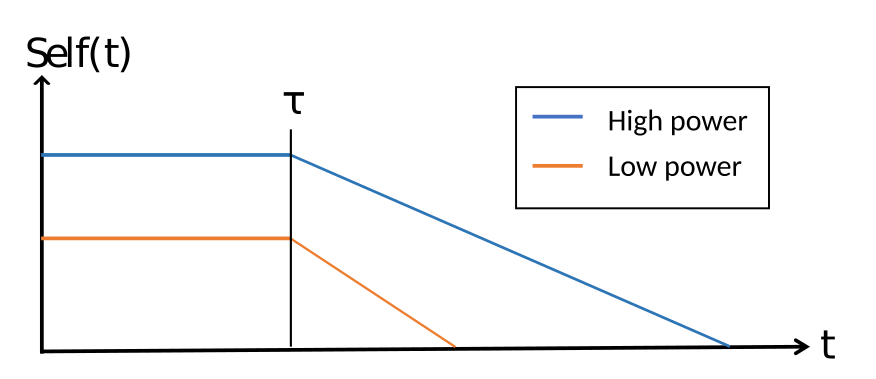
\includegraphics[width=2.2in]{graphs/s3.png}
			\caption{\label{fig:conc}Concession curve for self(t)}
		\end{floatingfigure} 
		
		In collaborative negotiation, both participants reduce their level of demand in time because they want to reach an agreement.
		According to our first principle, concessions should be higher for low-power agents. To implement this mechanism, we use a \emph{concession curve}, as illustrated on figure \ref{fig:conc}.
		
		This mechanism is defined as follows. Let $self(pow, t)$ be a time varying value, following the concession curve:
		
		\begin{equation}
		self(pow, t) = \left\{\begin{array}{ll}
		pow & \mathrm{if\ } (t \leq \tau)\\
		max(0, pow - (\frac{\delta}{pow} \cdot (t - \tau))) & \mathrm{otherwise}
		\end{array}\right.
		\end{equation}
		
		where is $t \geq 0$ is the number of open or rejected proposals, $\tau > 0$ is the minimum number of proposals before concession begins and $\delta > 0$ is a computational parameter of the concession slope. This value of $self$ represents the weight an agent gives to its self satisfaction relative to the other.
		
		The acceptability of a proposal of the dialogue $v \in C_i$ is defined as a boolean function:
		\vspace{-.5em} 
		\begin{equation}
		\vspace{-.5em} 
		acc(pow,v, t) = sat_{self}(v, \prec_i) \geq  \beta \cdot self(pow,t).
		\end{equation}
		with $\beta>0$ a parameter of the theory that defines the level of demand in function of the relation of power.
		
		This function is generalized to any option $o \in O$:
		\vspace{-.5em} 
		\begin{equation}
		acc(pow,o, t) = sat_{self}(o, \prec) \geq  \beta \cdot self(t)
		\vspace{-1.5em} 
		\end{equation}
		
		\subsubsection {Self vs other}
		According to our second principle, high-power negotiators give more weight to the satisfaction of their own preferences. To implement this principle in the context of collaborative negotiation, we compute how much a given proposal is \emph{tolerable} considering the satisfiability for both the agent and its interlocutor. The value returned by $tol$ is used to build proposals during the negotiation.
		
		For a given criteria $i\in\mathcal{C}$, let $V_i\subseteq C_i$ be the subset of values that are acceptable for the agent:
		\vspace{-1em} 
		\begin{equation}
		V_i(t) = \{ v\in C_i : acc(v,t) \}
		\vspace{-0.5em} 
		\end{equation}
		
		We compute the tolerability of a given value $v\in V_i$ at a time $t$ knowing the preference order $\prec_i$ and the preference of the interlocutor:
		\vspace{-1em} 
		\begin{equation}
		\begin{split}
		tol(v, t, \prec_i, A_i, U_i, pow) & = self(pow, t) . sat_{self}(v, \prec_i) \\
		& +  (1 - self(pow, t)) . sat_{other}(v, A_i, U_i)
		\end{split} 
		\end{equation}
		
		And we generalize this function to any option $o=(v_1,\ldots,v_n) \in O$:
		
		\begin{equation}
		tol(o, t, \prec, A, U, pow) = \frac{ \sum_{i}^{n} tol(v_i, t, \prec_i, A_i, U_i, pow) } {n}
		\end{equation}
		
		
		\subsubsection{Lead of the negotiation}
		According to our third principle, high-power negotiators tend to lead the negotiation. We implemented this principle through the choice of utterance types described on table \ref{utt}. An agent can express more than one utterance in a single turn.
		A high-power agent will focus on keeping the negotiation going by choosing \emph{negotiation moves} (ProposeValue /ProposeOption, RejectValue /RejectOption, AcceptValue/ AcceptOption). On the contrary, a lower power negotiator will focus on building an accurate model of other preferences in order to take the fairest decision. It will focus more on \emph{statement moves} (StateValue or AskValue/ AskCriterion).
		
		We define a threshold $\pi$ to split the spectrum of power in two. We describe on table \ref{utt} the rules for utterance selection. Depending on the power, the previous utterance $u^{-1}$ type and the current dialogue state, the agent will select the first utterance type for which the condition is satisfied. For instance, a high-power agent will stop the negotiation as soon as all the remaining options are unacceptable (line 2). A low-power agent will reject and state a preference, so as to explain why the proposal is not acceptable (line 14). If there is no open proposal, the low-power agent will ask for new information (line 18 -19). 
		
		\begin{table}[!t]
			{\scriptsize
				\centering
				\begin{tabular}{|p{.3cm}|p{.6cm}|p{3cm}|p{7.5cm}|}
					\hline
					\parbox[t]{2mm}{\multirow{5}{*}{\rotatebox[origin=c]{90}{\textbf{pow  $>\pi$}}}}&Line nb& \textbf{Utterance type} & \textbf{Condition} \\
					\cline{2-4}
					&1&NegotiationSuccess & $\exists o \in T\cup P$, $acc(pow,o,t)$ \\
					\cline{2-4}
					& 2& NegotiationFailure & $ \forall o \in \mathcal{O},  \neg acc(pow,o,t)$\\
					\cline{2-4}
					&3& StateValue(v) & $type(u^{-1}) = AskPreference \land n < \alpha$ \newline where $n$ is the number of successive statement moves\\
					\cline{2-4}
					&4& AcceptValue(v)+ \newline ProposeValue(c) & $ \exists v \in P_i$ / $acc(pow,v,t) \land \exists i\in\mathcal{C}, acc(pow,c,t)$ \\
					\cline{2-4}
					&5& AcceptValue(v)+\newline ProposeOption(o) &  $ \exists v \in P_i$ / $ acc(pow,v,t) \land \exists o \in \mathcal{O}$/ $ v \in o \land acc(pow,o,t)$ \\
					\cline{2-4}
					&6& RejectValue(v)+\newline ProposeValue(c) & $ \exists v \in P_i$ / $ \neg acc(pow,v,t) \land \exists i\in\mathcal{C}, acc(pow,c,t)$ \\
					\cline{2-4}
					&7& RejectValue(v)+ \newline ProposeOption(o) &  $ \exists v \in P_i$ / $  \neg acc(pow,v,t) \land \exists o \in \mathcal{O}$/ $acc(pow,o,t)$ \\
					\cline{2-4}
					& 8&RejectOption($o_1$)+ ProposeOption($o_2$) & $ \exists o_1 \in P$ / $ \neg acc(pow,o_1,t) \land \exists o_2\in\mathcal{O}, acc(pow,o_2,t)$ \\
					\cline{2-4}
					&9& ProposeValue(v) & $\exists v \in C_i$ / $tol(v, t, \prec_i, A_i, U_i, pow)$\\
					\cline{2-4}
					&10& ProposeOption(o) & $\exists o \in \mathcal{O}$ / $tol(o, t, \prec_i, A_i, U_i, pow)$\\
					
					\hline
					
					\parbox[t]{2mm}{
						\multirow{5}{*}{\rotatebox[origin=c]{90}{ \textbf{pow  $ \leq \pi$}}}} & 11& Negotiation success &  $\exists o \in T$ \\
					\cline{2-4}
					&12& AcceptValue(v) & $\exists i\in\mathcal{C}, \exists v \in P_i, acc(pow, v, t)$ \\
					\cline{2-4}
					&13&AcceptOption(o) & $\exists o \in P, acc(pow, o, t)$ \\
					\cline{2-4}
					&14&RejectValue(v)+\newline StateValue(v) & $ t<\tau \land (\exists i\in\mathcal{C}, \exists v \in P_i, \neg acc(pow,v, t))$.\\
					\cline{2-4}
					&15&RejectOption(o)+ \newline StateValue(v) & $ t<\tau \land (\exists o \in P,  \neg acc(pow,o, t) \land \exists v \in o, \neg acc(pow,v, t))$.\\
					\cline{2-4}
					&16&ProposeValue(v) &  $\exists i\in\mathcal{C}, \exists v \in C_i, v \in A_i  \land acc(pow, v, t) $\\
					\cline{2-4} 
					&17&ProposeOption(o)  & $\forall i\in\mathcal{C},\exists v \in C_i, v \in T_i  \land v \in o$ \\
					\cline{2-4} 
					&18&AskValue(v) & $t > \tau \land \exists i\in\mathcal{C}, \exists c \in P_i, \neg acc(c, t)$ \\
					\cline{2-4} 	
					&19&AskCriterion(i) & $\exists i\in\mathcal{C}, A_i \cup U_i= \emptyset $\\
					\cline{2-4}	
					&20&StateValue(v) & $\exists i\in\mathcal{C}, C_i\cap S_i \neq \emptyset$	\\
					\cline{2-4}
					&21& ProposeValue(v) & $\exists v \in C_i$ / $tol(v, t, \prec_i, A_i, U_i, pow)$\\
					\cline{2-4}
					&22& ProposeOption(o) & $\exists o \in \mathcal{O}$ / $tol(o, t, \prec_i, A_i, U_i, pow)$\\
					
					\hline
				\end{tabular}
			}
			\caption{Selection of utterance types}
			\label{utt}
		\end{table}
		
		\section{Evaluation}
		\label{sec:evaluation}
		
		In order to validate our model, we conducted a perceptual study in which participants have to determine the behaviors of two agents generated using our model. We have implemented the model in Java with the DISCO platform \cite{rich09} and we generated synthetic dialogues between two artificial agents with different values of power and preferences.
		
		\subsection{Study design}
		We simulate a collaborative negotiation for choosing a restaurant. We built a set of four criteria (cuisine, ambiance, price and location) for a total of 420 options. An example of dialogue is given in figure \ref{fig:ex-dialogue}. The following parameter values were used in our simulation: $\tau=2$, $\pi=0.5$, $\alpha=2$, $\beta=1$ and $\delta=0.1$. We generated three preferences sets and we measured the difference between the preference sets using Kendall's distance \cite{bra2013Kendall}. We manipulated two simulation parameters: the power of both agents (named \emph{pow-a} and \emph{pow-b}) and the preference sets. This later affects the generation of dialogues in term of values and lengtht.  Table \ref{table:conditions} summarizes the 4 experimental conditions that results from this combination. Note that we only consider one configuration of social power for the similar preference sets condition, because the resulting dialogues are very similar. The first speaker (Speaker A) is always the high-power agent, as stated by our principle 3 on leading the dialogue.
		
		Our goal is to show these dialogues to human observers so as to evaluate how the relation pf power is perceived in the different dialogues.
		\begin{table}
			\centering
			\begin{tabular}{ |l|c|c|l| }
				\hline
				\textbf{Preferences}& \textbf{pow-a} & \textbf{pow-b} & \textbf{Label} \\ 
				\hline
				\newline\multirow{3}{*} {Different preferences (Kendall's tau = $0.96$)} & 0.9 & 0.4 & Dialogue 1 \\ \cline{2-4}
				
				\newline  & 0.7 & 0.4 & Dialogue 2\\ \cline{2-4}
				
				\newline   &0.7 & 0.2 & Dialogue 3\\ 
				\hline
				\newline Similar preferences (Kendall's tau = $0.46$) & 0.7 & 0.4 & Dialogue 4\\
				\hline
			\end{tabular}
			\caption{Initial condition's setting for generating dialogues} 
			\label{table:conditions}
		\end{table}
		
		
		\begin{figure}
			\fbox{\begin{minipage}{.95\textwidth}
					{\scriptsize\ttfamily
						\begin{addmargin}[1em]{2em}% 1em left, 2em right
							A: "Let's go to a Chinese restaurant."
							
							\hspace*{3mm}B: "I don't like Chinese restaurants, let's choose something else."
							
							A: "Let's go to a cheap restaurant."
							
							\hspace*{3mm}B: "Do you like expensive restaurants?"
							
							A: "I don't like expensive restaurants."
							
							($\ldots$)
							
							\hspace*{3mm}B: "What kind of atmosphere do you like?"
							
							A: "Let's go to a cheap restaurant."
							
							\hspace*{3mm}B: "Okay, let's go to a cheap restaurant."
							
							A: "Let's go to Sap. It's a quiet, cheap Japanese restaurant on the south side."
							
							\hspace*{3mm}B: "Okay, let's go to Sap.
						\end{addmargin}
					}
				\end{minipage}}
				
				\caption{\label{fig:ex-dialogue}Excerpt of Dialogue 2.}
			\end{figure}
			\vspace{-1em} 
			\subsection{Hypotheses}
			\vspace{-.5em} 
			Based on our three principles and the literature in on the perception of social power in negotiation, we investigated four hypotheses:
			\vspace{-.5em} 
			\begin{itemize}
				\item  \textbf{H1:} The high-power speaker will more strongly be perceived as self-centered than the lower power speaker.  
				
				\item \textbf{H2:} The low-power speaker will be more strongly perceived as making larger concessions than the higher-power speaker.
				
				\item \textbf{H3:}  The high-power speaker will more strongly be perceived as having a higher level of demand than to the low-power speaker.
				
				\item \textbf{H4:}  The high-power speaker will more strongly be perceived as taking the lead in the negotiation than the low-power speaker.
				
			\end{itemize}
			
			
			\subsection{Experimental Procedure}
			
			We conducted a between-subject study using the online crowdsoursing website \emph{CrowdFlower}\footnote{https://www.crowdflower.com/}. 
			Each participant was shown only one dialogue. Agents were described as two friends trying to find a restaurant where to have dinner. %We wanted to avoid skewing the participant's perception by the fact that negotiators are artificial agents. 
			Participants were invited to read the assigned dialogue and answer a questionnaire. 
			
			We defined two questions for each hypothesis. Two sanity-check questions were added. Each one of these questions was to be answered on a 5 points Likert scale ranging from "I totally disagree" to "I totally agree".
			
			\begin{table}
				{\scriptsize
					\begin{tabular}{|p{1.75cm}|p{5cm}|p{5.5cm}|}
						\hline
						Hypothesis &question 1& question 2 \\
						\hline
						\textbf{H1} &Speaker (A/B) is self-centered. &Speaker (A/B) takes his friend's preferences into account in the choice of the restaurant.\\
						\hline
						\textbf{H2} &Speaker (A/B) makes concessions in the negotiation.&Speaker (A/B) gives up his position in the negotiation\\
						\hline
						\textbf{H3} & Speaker (A/B) is demanding&Speaker (A/B) presses his position in the negotiation. \\
						\hline
						\textbf{H4} &Speaker (A/B) takes the lead in the negotiation.&Speaker (A/B) takes the initiative in the negotiation \\
						\hline
					\end{tabular}
				}
				\caption{List of questions asked for the questionnaire}
				\label{table:questionnaire}
			\end{table}
			\vspace{-1em} 
			A total of 120 native English subjects participated to the experiment (30 for each condition). Each subject received \textit{25 cents} and we excluded 15 participants after sanity check.
			
			\subsection{Results and discussion}
			\vspace{-.5em} 
			Table  \ref{res} summarizes the results of our study, which strongly support all of our four hypotheses: in each dialogue, the high-power agent and the low-power agent were clearly distinguished on all aspects. We first computed the correlation for each pair of questions (the average correlation is at .5 for all pairs of questions in all dialogues). This permits us to use the data to compare the speakers behavior on each dialogue. Since our data are not normally distributed, we used a non parametric Wilcoxon signed-rank test for paired data. The high-power speaker was correctly perceived as more self-centered (\textbf{H1}), making less concessions (\textbf{H2}), having a higher level of demand (\textbf{H3}) and leading the negotiation (\textbf{H4}).
			\subsubsection{Interpersonal nature of power}
			Finally, we made a post-study analysis by comparing the participant's judgments on the behaviors of Speaker A across different dialogues. Our hypothesis was that a greater difference in power would lead to a better perception of behaviors related to power. We computed the differences between the evaluations of Speakers A and B in Dialogue 1 and Dialogue 2 (pow-b remains unchanged at 0.4 whereas pow-a changes from 0.7 to 0.9). We did not obtain significant results, however, a tendency was observed ($p\simeq 0.1$) for self-centeredness, concessions and the lead of dialogue was clearly better perceived ($p=0.043$). This lack of result might be explained by the interpersonal nature of power, which means that participants rate the power of Speaker A as opposed to the behavior of Speaker B, which makes the comparison of agents behaviors from different dialogues partly irrelevant.
			
			\subsubsection{Limitations}
			In this present experiment, we studied the perception of all the principles related to power simultaneously. One of the limits of this study concerns the fact that we did not investigate the perception of each principle individually. \hl{However, due to the fact that the principles are interdependent, an independent evaluation would be difficult. (MAL DIT)}
			
			\begin{table}[t]
				{\scriptsize
					\begin{tabular}{|ll|c|c|c|c|c|c|c|c|} 
						\cline{3-10}
						
						\multicolumn{1}{c} {}	& \multirow{2}{*} {}& \multicolumn{2}{c|} {Dialogue1} & \multicolumn{2}{c|} {Dialogue2} & \multicolumn{2}{c|} {Dialogue3} &\multicolumn{2}{c|} {Dialogue4} \\ 
						\cline{3-10}
						
						
						\multicolumn{1}{c} {} & & SpeakerA & SpeakerB & SpeakerA & SpeakerB & SpeakerA & SpeakerB & SpeakerA & SpeakerB \\
						\hline 
						%\multicolumn{9}{|c|}{ \textbf{Results for H1}} \\
						%	\hline
						\newline \multirow{2}{*} {\textbf{H1}}  & \multicolumn{1}{|l|}{ \textit{Mean} $\pm$ \textit{SD} } & 3.9 $\pm$ 1.1 & 2.2$\pm$ 0.9  & 3.6 $\pm$0.9 & 2.2 $\pm$0.8  &2.8 $\pm$1.1  & 2.13$\pm$ 0.7 & 3.4 $\pm$ 1 & 2 $\pm$0.9 \\
						\cline{2-10}	
						\newline & \multicolumn{1}{|l|}{p-value} & \multicolumn{2}{c|}{ $<<0.01$} & \multicolumn{2}{c|}{ $<<0.01$} & \multicolumn{2}{c|}{ $<0.01$}& \multicolumn{2}{c|}{ $<<0.01$}\\
						\hline	
						
						\newline \multirow{2}{*} {\textbf{H2}} &\multicolumn{1}{|l|}{ \textit{Mean} $\pm$ \textit{SD} } & 2.2 $\pm$ 1.1 & 4.3$\pm$ 0.8  & 2.5 $\pm$1.2 & 3.8 $\pm$1.04 &2.7 $\pm$1.2  & 3.6$\pm$ 0.8 & 2.3 $\pm$ 1 & 3.2 $\pm$1.2 \\
						\cline{2-10}	
						\newline & \multicolumn{1}{|l|}{p-value} & \multicolumn{2}{c|}{ $<<0.01$} & \multicolumn{2}{c|}{ $<<0.01$} & \multicolumn{2}{c|}{ $=0.01$}& \multicolumn{2}{c|}{ $<<0.01$}\\
						\hline	
						
						\newline \multirow{2}{*} {\textbf{H3}} &\multicolumn{1}{|l|}{ \textit{Mean} $\pm$ \textit{SD} } & 4.1 $\pm$ 0.8 & 2.6$\pm$ 1.1 & 4.03 $\pm$ 0.8 & 2.7 $\pm$0.9 &3.5 $\pm$1.1 & 2.3$\pm$ 1 & 3.8 $\pm$ 1.8 & 1.8 $\pm$0.8 \\
						\cline{2-10}	
						\newline & \multicolumn{1}{|l|}{p-value}  & \multicolumn{2}{c|}{ $<<0.01$} & \multicolumn{2}{c|}{ $<<0.01$} & \multicolumn{2}{c|}{ $<0.01$}& \multicolumn{2}{c|}{ $<<0.01$}\\
						\hline	
						%				
						
						
						\newline \multirow{2}{*} {\textbf{H4}} & \multicolumn{1}{|l|}{ \textit{Mean} $\pm$ \textit{SD} } & 4.2 $\pm$ 0.9 & 2.3$\pm$ 1.1  & 3.8 $\pm$0.9 & 2.6 $\pm$1.07 & 3.8 $\pm$0.9  & 2.8$\pm$ 1.1  & 4.5 $\pm$0.5  & 1.9 $\pm$ 0.9\\
						\cline{2-10}
						\newline & \multicolumn{1}{|l|}{p-value} & \multicolumn{2}{c|}{ $<<0.01$} & \multicolumn{2}{c|}{ $<<0.01$} & \multicolumn{2}{c|}{ $<0.05$}& \multicolumn{2}{c|}{ $<<0.01$}\\
						\hline	
					\end{tabular}
				}
				\caption{Summary of the obtained results for each hypothesis}
				\label{res}
			\end{table}
			
			\subsection{Conclusion}
			
			Our research aims to model a conversational agent which is able to deploy different strategies of negotiation depending on its representation of social power. Based on research in social psychology, we defined three principles of behaviors related to power in collaborative negotiation. We proposed a model of utterance selection based on modeling of preferences and the implementation of these principles. We showed that the behaviors related to social power are correctly perceived in the resulting dialogues. Our findings validate our model of dialogue in general and specifically confirmed the coherence of the generated behaviors of power.
			
			Our next study will focus on using this model in a human-agent interaction. It was proven by \cite{klatt2011negotiations} that having a model of the other impacts the negotiation strategy and improves the outcomes. Therefore, we aim to use our dialogue model to build a representation of the interlocutor's social power, following a theory of mind approach. We would like to show that an agent that adapts its own strategy to the perceived power of its interlocutor makes a better collaborative negotiator.		
			
			
			% ================== BIBLIO ===============
			
			\scriptsize{	
				\bibliographystyle{plain}
				\bibliography{Library}}
			
			
			
		\end{document}